\documentclass{article}

% ============================================================
% TEMPLATE DO PROJETO DESENVOLVIDO (ETAPA 2)
% Adaptado do template oficial do NeurIPS 2026 para uso na disciplina.
%
% INSTRUÇÕES PARA OS ALUNOS:
% - Baixe também o arquivo neurips_2026.sty do template original em:
%   https://www.overleaf.com/latex/templates/formatting-instructions-for-neurips-2026/bjdwqfdkyftc
% - LIMITE DE PÁGINAS DESTA ETAPA: tentem manter entre 4 a 6 páginas, sem contar as referências, figuras e tabelas. 
% - Este documento parte da proposta (Etapa 1): reaproveitem e atualizem
%   as seções Introduction, Related Work, Data e Methodology conforme o
%   que de fato foi feito, e acrescentem os resultados obtidos.
% - Não é necessário anonimizar o documento nem incluir checklist.
% ============================================================

\usepackage[preprint]{neurips_2026}

\usepackage[utf8]{inputenc}
\usepackage[T1]{fontenc}
\usepackage{hyperref}
\usepackage{url}
\usepackage{booktabs}
\usepackage{amsfonts}
\usepackage{amsmath}
\usepackage{nicefrac}
\usepackage{microtype}
\usepackage{xcolor}
\usepackage{graphicx}
\graphicspath{{../../results/figures/}}

\title{Avaliação Comparativa da Fidelidade de Métodos de Explicabilidade em Modelos de Classificação de Imagens: Vision GNNs vs.\ Vision Transformers}

\author{%
  Henrique Coelho Beltrão \\
  Código: B435909 \\
  \texttt{riquecbeltrao@hotmail.com} \\
}
\begin{document}

\maketitle

\begin{abstract}
Comparamos a fidelidade de métodos de explicabilidade \textit{post-hoc} (Grad-CAM, Attention Rollout, LIME, Partition SHAP e Integrated Gradients) entre uma Vision GNN isotrópica (\textbf{ViG-Ti}) e um Vision Transformer (\textbf{DeiT-Tiny}) no \textit{dataset} Imagenette2-160. Em FP32 estrito, ambos atingem acurácia pareada no teste ($97{,}20\%$ vs.\ $96{,}94\%$; $97/100$ na amostra de XAI). Em $N = 100$ imagens, o Grad-CAM na ViG-Ti supera o Grad-CAM e o Rollout do DeiT-Tiny em Deletion/Insertion AUC ($p \le 0{,}0085$). O Rollout falha no \textit{sanity check} do cabeçalho (Spearman $1{,}000$), enquanto o DeiT-Tiny lidera em Integrated Gradients (Insertion $0{,}879$ vs.\ $0{,}684$) e robustez a ruído, o Partition SHAP exibe maior consistência cruzada e a oclusão por preto induz \textit{graph rewiring} precoce na ViG-Ti. Conclui-se que a conectividade em grafo $k$-NN dinâmico altera sistematicamente a fidelidade frente ao \textit{self-attention} denso.
\end{abstract}

\section{Introduction}
\label{sec:intro}
% Atualizem a introdução da proposta, se necessário. Mantenham a
% pergunta de pesquisa e os objetivos, ajustando caso o escopo do
% projeto tenha mudado ao longo do desenvolvimento.

Métodos de \textit{Explainable AI} (XAI) \textit{post-hoc} produzem mapas locais de atribuição para modelos de visão computacional sem alterar seu treinamento. Contudo, explicadores distintos geram mapas divergentes para a mesma predição, exigindo métricas que distingam plausibilidade visual de fidelidade (\textit{faithfulness}) ao funcionamento interno da rede.

Comparações tradicionais entre CNNs e Vision Transformers (ViTs) misturam hierarquia espacial, campos receptivos locais e número de parâmetros. Para isolar o mecanismo de agregação espacial, comparamos duas arquiteturas isotrópicas equivalentes em grade ($14 \times 14 = 196$ nós/\textit{tokens}), profundidade ($12$ blocos), largura ($D = 192$) e custo ($1{,}3\text{B}$ FLOPs): o \textbf{DeiT-Tiny} \citep{dosovitskiy2021vit,touvron2021deit}, que modela a imagem como grafo completo via \textit{self-attention}, e a \textbf{ViG-Ti} \citep{han2022vig}, que opera por \textit{message passing} sobre um grafo $k$-NN dinâmico no espaço de \textit{features}.

\textbf{Pergunta de pesquisa:} \textit{métodos de XAI post-hoc (Grad-CAM, Attention Rollout, LIME, Partition SHAP e Integrated Gradients) mantêm o mesmo nível de fidelidade, sanidade paramétrica e estabilidade ao comparar uma Vision GNN (ViG-Ti) e um Vision Transformer (DeiT-Tiny) na mesma tarefa?}

\textbf{Objetivos executados:} (1) \textit{fine-tuning} controlado no Imagenette2-160 (\textbf{E1}); (2) geração dos mapas em amostra estratificada fixa de $N = 100$ imagens (\textbf{E2}); (3) avaliação de Deletion/Insertion AUC com testes de Wilcoxon (\textbf{E3}); (4) \textit{sanity checks} por aleatorização em cascata (\textbf{E4}); (5) medição de \textit{graph rewiring} na ViG-Ti (\textbf{E5}); e (6) teste de robustez a ruído gaussiano (\textbf{E6}) e ablações de hiperparâmetros. O trabalho integra \textit{Explainable AI}, \textit{Self-Attention} e \textit{Graph Neural Networks}.

\section{Related Work}
\label{sec:related}
% Atualizem a revisão da proposta com trabalhos adicionais encontrados
% ao longo do desenvolvimento, se houver.

\textbf{ViG e Vision Transformers.} \citet{dosovitskiy2021vit} introduziram o ViT com \textit{self-attention} global sobre \textit{patches}, tornado eficiente em dados pelo DeiT \citep{touvron2021deit}. \citet{darcet2024registers} observaram que ViTs sem \textit{register tokens} concentram norma elevada em \textit{tokens} de fundo e borda. Generalizando grades e sequências para grafos, \citet{han2022vig} propuseram a ViG com grafo $k$-NN dinâmico, convolução \textit{Max-Relative} (\textit{Grapher}) e módulos FFN.

\textbf{Explicabilidade nativa, agnóstica e avaliação.} \citet{pope2019gnn} adaptaram o Grad-CAM \citep{selvaraju2017gradcam} para nós de GNNs, abordagem adotada aqui no lugar do GNNExplainer \citep{ying2019gnnexplainer} por permitir comparação direta na grade $14 \times 14$ contra os \textit{tokens} do DeiT-Tiny. Para ViTs, o Attention Rollout \citep{abnar2020rollout} agrega atenção entre camadas, embora não seja específico à classe \citep{chefer2021transformer}. Incluímos ainda LIME \citep{ribeiro2016lime}, Partition SHAP \citep{lundberg2017shap} e Integrated Gradients \citep{sundararajan2017ig}, avaliados via Deletion/Insertion AUC \citep{petsiuk2018rise} (alternativa sem retreino ao ROAR \citep{hooker2019roar}) e \textit{sanity checks} de aleatorização \citep{adebayo2018sanity}.

\section{Data}
\label{sec:data}
% Descrevam os dados efetivamente usados (podem diferir do que foi
% planejado na proposta) e o pré-processamento efetivamente aplicado.
% Se algo mudou em relação à proposta, expliquem por quê.

Utilizou-se o \textit{dataset} \texttt{imagenette2-160} ($13.394$ imagens JPEG em $10$ classes do ImageNet, convertidas para RGB). Para evitar vazamento de dados, o treino oficial ($9.469$ imagens) foi usado no \textit{fine-tuning}, e a validação oficial ($3.925$ imagens) foi particionada estratificadamente (\texttt{seed=42}) em $80\%$ para validação ($3.140$) e $20\%$ para teste intocado ($785$). Do teste, extraiu-se deterministicamente a amostra fixa de $N = 100$ imagens ($10$ por classe, \texttt{xai\_subset.csv}), com interseção nula entre treino, validação e teste.

As imagens são redimensionadas para $224 \times 224$ (interpolação bicúbica), com \textit{RandomResizedCrop} $(0{,}8,\,1{,}0)$ e \textit{RandomHorizontalFlip} ($p = 0{,}5$) apenas no treino. Em vez da normalização $(0{,}5,\,0{,}5,\,0{,}5)$ original da ViG-Ti, ambos os modelos usaram a média e o desvio-padrão do ImageNet, padronizando as entradas e \textit{baselines} de XAI.

\section{Methodology}
\label{sec:method}
% Descrevam o método/modelo efetivamente implementado. Se ele mudou em
% relação à proposta, expliquem as razões da mudança.

\textbf{Modelos comparados:} o \textbf{DeiT-Tiny} (\texttt{timm}, $5.526.346$ parâmetros) possui $12$ blocos de \textit{self-attention} ($3$ cabeças) e MLP sobre $196$ \textit{tokens} ($D = 192$). A \textbf{ViG-Ti} (\texttt{vig\_pytorch} adaptado para PyTorch 2.15/\texttt{timm} 1.0, pesos \texttt{vig\_ti\_74.5.pth}, $6.169.994$ parâmetros) possui um \textit{Stem} de $5$ convoluções $3 \times 3$ e $12$ blocos \textit{Grapher}+\texttt{FFN} com \texttt{MRConv2d} sobre grafo $k$-NN dilatado ($k$ de $9$ a $18$; dilatação $d \in \{1, 2, 3\}$ nos blocos $0$ a $3$, $4$ a $7$ e $8$ a $11$).

\textbf{Instrumentação e precisão FP32:} no DeiT-Tiny, apenas o \textit{token} \texttt{CLS} segue ao cabeçalho final, anulando gradientes após \texttt{blocks[-1]}; portanto, o \textit{hook} de Grad-CAM foi colocado em \texttt{blocks[-1].norm1} com reconstrução espacial $(B, 192, 14, 14)$. No Rollout, desabilitou-se \texttt{fused\_attn} apenas na coleta de \texttt{attn\_drop} (diferença máxima nos logits de $8{,}50 \times 10^{-7}$). Na ViG-Ti, variações numéricas de TF32 entre tamanhos de lote trocavam vizinhos discretos no \texttt{topk} em $1/100$ imagem; desabilitar TF32 (\texttt{allow\_tf32=False}) restaurou $100/100$ de concordância entre $B = 1$, $32$ e $64$.

\textbf{Métodos de XAI:} os mapas explicam a classe prevista ($\arg\max$) e são normalizados para $[0, 1]$: (1) \textbf{Grad-CAM} \citep{selvaraju2017gradcam,pope2019gnn} na grade $14 \times 14$ final (\texttt{backbone[-1]} na ViG-Ti; \texttt{blocks[-1].norm1} no DeiT-Tiny) com \texttt{ReLU} e interpolação bilinear; (2) \textbf{Attention Rollout} \citep{abnar2020rollout} no DeiT-Tiny via média das cabeças e $(0{,}5\,A + 0{,}5\,I)$ nos $12$ blocos (\texttt{discard\_ratio} $= 0$); (3) \textbf{LIME} \citep{ribeiro2016lime} com $1000$ amostras, \texttt{hide\_color} $= 0$, probabilidades \textit{softmax} e SLIC (\texttt{n\_segments} $= 50$, \texttt{compactness} $= 10$); (4) \textbf{Partition SHAP} \citep{lundberg2017shap} com \texttt{max\_evals} $= 500$ sobre \textbf{logits brutos} (evitando saturação do \textit{softmax}) e \textit{masker} \texttt{blur(32,32)} via filtro uniforme $32 \times 32$; e (5) \textbf{Integrated Gradients (IG)} \citep{sundararajan2017ig} com $m = 50$ passos (\texttt{riemann\_right}) a partir do \textit{baseline} preto normalizado $x'$ e soma dos valores absolutos nos canais:
\begin{equation}
    \mathrm{IG}_i(x) = (x_i - x_i') \times \frac{1}{m}\sum_{k=1}^{m} \frac{\partial F\left(x' + \frac{k}{m}(x - x')\right)}{\partial x_i}.
\end{equation}
Ressalta-se que o Grad-CAM é específico à classe, enquanto o Rollout é agnóstico à classe \citep{chefer2021transformer}.

\section{Experiments}
\label{sec:exp}
% O que escrever aqui:
% - Desenho experimental efetivamente executado.
% - Baselines usados na comparação.
% - Métricas de avaliação usadas.
% - Detalhes de implementação relevantes para reprodutibilidade
%   (hiperparâmetros, hardware, tempo de treinamento, splits de dados).

Executou-se toda a pipeline em GPU \texttt{RTX 4070 Laptop} (8 GiB), Python \texttt{3.13.12}, PyTorch \texttt{2.15.0+cu132}, \texttt{seed=42} e FP32 estrito:

\textbf{E1 e E2 (Treino e mapas):} \textit{fine-tuning} por $15$ épocas (\texttt{AdamW}, \texttt{lr} $= 10^{-4}$, \texttt{weight\_decay} $= 10^{-2}$, \texttt{batch\_size} $= 32$, \textit{warmup} de $1$ época e decaimento cosseno até $10^{-6}$, paciência $5$ não acionada) com seleção pelo melhor \texttt{val\_acc}. Em E2, os $9$ pares modelo $\times$ método foram persistidos em \texttt{.npz} para $N = 100$ ($876{,}9\text{ s}$ acumulados; $100/100$ de acordo com E1).

\textbf{E3 (Fidelidade):} curvas de Deletion e Insertion AUC em $50$ passos ($0\%$ a $100\%$) sob \textit{baselines} \texttt{black} e \texttt{blur} ($21 \times 21$, $\sigma = 10{,}0$) em $N = 100$, com desempate determinístico contra saliência uniforme aleatória (\texttt{random}) e $60$ testes pareados de Wilcoxon.

\textbf{E4, E5, E6 e ablações:} em E4, aplicou-se aleatorização em cascata em $6$ estágios (\texttt{head}, blocos \texttt{9\_11} a \texttt{0\_11} e \texttt{all\_layers}, reinicializando também \texttt{pos\_embed} e \texttt{cls\_token}), medindo Spearman e SSIM ($N = 100$ para Grad-CAM/Rollout/IG; $N = 20$ estratificado com $2$/classe para LIME/SHAP; $1.426{,}6\text{ s}$). Em E5, mediu-se retenção, taxa de \textit{rewiring} ($1 - \text{retenção}$) e distância de Jaccard nas arestas $k$-NN da ViG-Ti em $20$ passos de Deletion (Bloco 11 e perfil nos $12$ blocos em $20\%$ e $50\%$, $N = 100$). Em E6, adicionou-se ruído gaussiano ($\sigma \in \{0{,}02,\,0{,}05,\,0{,}10\}$ em $[0, 1]$, $696{,}3\text{ s}$) para medir Spearman, SSIM e troca de predição. Nas ablações ($N = 20$, $385{,}2\text{ s}$), variaram-se \texttt{n\_segments} $\in \{25, 50, 100\}$ (LIME) e \texttt{n\_steps} $\in \{20, 50, 100\}$ (IG).

\section{Results}
\label{sec:results}
% O que escrever aqui:
% - Apresentem os resultados obtidos de forma objetiva (tabelas, figuras,
%   gráficos). Ver exemplos de tabela e figura comentados abaixo.
% - Não interpretem os resultados aqui — isso vai na seção Discussion.

% \begin{table}[h]
%   \caption{Resultados obtidos no conjunto de teste.}
%   \label{tab:results}
%   \centering
%   \begin{tabular}{lcc}
%     \toprule
%     Método & Métrica 1 & Métrica 2 \\
%     \midrule
%     Baseline & & \\
%     Proposto & & \\
%     \bottomrule
%   \end{tabular}
% \end{table}

% \begin{figure}[h]
%   \centering
%   \includegraphics[width=0.7\linewidth]{resultados.pdf}
%   \caption{Descrição do que a figura mostra e principal conclusão.}
%   \label{fig:results}
% \end{figure}

\textbf{Desempenho e tempos (E1 e E2):} conforme a Tabela~\ref{tab:e1}, ViG-Ti e DeiT-Tiny atingem paridade no teste ($97{,}20\%$ vs.\ $96{,}94\%$) e empatam em $97/100$ no \texttt{xai\_subset} ($96$ acertos conjuntos, $1$ exclusivo por modelo e $2$ erros conjuntos), com treino $2{,}3\times$ mais rápido no DeiT-Tiny. Em E2, os tempos médios por imagem foram $0{,}020\text{ s}$ vs.\ $0{,}008\text{ s}$ (Grad-CAM), $0{,}006\text{ s}$ (Rollout), $0{,}220\text{ s}$ vs.\ $0{,}118\text{ s}$ (IG), $1{,}615\text{ s}$ vs.\ $0{,}892\text{ s}$ (Partition SHAP) e $3{,}720\text{ s}$ vs.\ $2{,}169\text{ s}$ (LIME).

\begin{table}[t]
  \caption{Desempenho de \textit{fine-tuning} e avaliação em FP32 estrito no Imagenette2-160 (E1).}
  \label{tab:e1}
  \centering
  \footnotesize
  \setlength{\tabcolsep}{4.5pt}
  \begin{tabular}{lcccccccc}
    \toprule
    Modelo & Params & Melhor Época & Treino (s) & Val Loss & Val Acc & Test Loss & Test Acc & Test F1 \\
    \midrule
    ViG-Ti    & $6{,}17\text{M}$ & 12 & $814{,}8$ & $0{,}0599$ & $98{,}50\%$ & $0{,}0765$ & $97{,}20\%$ & $0{,}9720$ \\
    DeiT-Tiny & $5{,}53\text{M}$ & 14 & $354{,}9$ & $0{,}0864$ & $97{,}64\%$ & $0{,}1133$ & $96{,}94\%$ & $0{,}9694$ \\
    \bottomrule
  \end{tabular}
\end{table}

\textbf{Fidelidade via Deletion/Insertion AUC (E3):} a Tabela~\ref{tab:e3} e a Figura~\ref{fig:e3_auc} mostram que, sob \texttt{blur} e \texttt{black}, o Grad-CAM da ViG-Ti supera o Grad-CAM (Wilcoxon $p \le 2{,}65 \times 10^{-9}$) e o Attention Rollout ($p \le 8{,}53 \times 10^{-3}$) do DeiT-Tiny nas quatro métricas. No DeiT-Tiny, o Rollout supera o Grad-CAM em Insertion (\texttt{blur} $p = 1{,}21 \times 10^{-3}$; \texttt{black} $p = 1{,}67 \times 10^{-5}$) e Deletion \texttt{black} ($p = 3{,}54 \times 10^{-4}$). No IG, o DeiT-Tiny supera a ViG-Ti em Insertion AUC (\texttt{blur} $p = 1{,}22 \times 10^{-10}$; \texttt{black} $p = 1{,}04 \times 10^{-15}$). Na ViG-Ti sob \texttt{black}, \texttt{random} obtém Deletion AUC inferior (melhor) ao de todos os explicadores reais ($p < 2 \times 10^{-4}$), invertendo-se sob \texttt{blur} para Grad-CAM ($p = 8{,}99 \times 10^{-5}$) e Partition SHAP ($p = 0{,}0189$). Em oclusão total por \texttt{blur}, a probabilidade residual média é $0{,}517$ no DeiT-Tiny contra $0{,}271$ na ViG-Ti.

\begin{table}[t]
  \caption{Métricas de fidelidade (média $\pm$ DP em $N = 100$, E3). Valores em negrito indicam o melhor método real por coluna e modelo.}
  \label{tab:e3}
  \centering
  \resizebox{\linewidth}{!}{%
  \begin{tabular}{llcccc}
    \toprule
    Modelo & Método & Del AUC (\texttt{blur}) $\downarrow$ & Ins AUC (\texttt{blur}) $\uparrow$ & Del AUC (\texttt{black}) $\downarrow$ & Ins AUC (\texttt{black}) $\uparrow$ \\
    \midrule
    ViG-Ti & Grad-CAM & $\mathbf{0{,}461 \pm 0{,}263}$ & $0{,}914 \pm 0{,}095$ & $0{,}285 \pm 0{,}208$ & $0{,}784 \pm 0{,}177$ \\
    ViG-Ti & LIME & $0{,}577 \pm 0{,}269$ & $0{,}914 \pm 0{,}098$ & $\mathbf{0{,}266 \pm 0{,}158}$ & $0{,}866 \pm 0{,}114$ \\
    ViG-Ti & Partition SHAP & $0{,}481 \pm 0{,}265$ & $\mathbf{0{,}947 \pm 0{,}077}$ & $0{,}432 \pm 0{,}229$ & $\mathbf{0{,}899 \pm 0{,}099}$ \\
    ViG-Ti & Integrated Gradients & $0{,}662 \pm 0{,}241$ & $0{,}684 \pm 0{,}208$ & $0{,}323 \pm 0{,}242$ & $0{,}393 \pm 0{,}237$ \\
    ViG-Ti & Random (controle) & $0{,}542 \pm 0{,}265$ & $0{,}547 \pm 0{,}256$ & $0{,}219 \pm 0{,}212$ & $0{,}225 \pm 0{,}213$ \\
    \midrule
    DeiT-Tiny & Grad-CAM & $0{,}725 \pm 0{,}292$ & $0{,}782 \pm 0{,}221$ & $0{,}556 \pm 0{,}270$ & $0{,}601 \pm 0{,}251$ \\
    DeiT-Tiny & Attention Rollout & $0{,}672 \pm 0{,}286$ & $0{,}851 \pm 0{,}183$ & $0{,}459 \pm 0{,}239$ & $0{,}735 \pm 0{,}220$ \\
    DeiT-Tiny & LIME & $0{,}644 \pm 0{,}287$ & $0{,}905 \pm 0{,}142$ & $0{,}285 \pm 0{,}160$ & $\mathbf{0{,}892 \pm 0{,}099}$ \\
    DeiT-Tiny & Partition SHAP & $\mathbf{0{,}445 \pm 0{,}287}$ & $\mathbf{0{,}956 \pm 0{,}065}$ & $0{,}395 \pm 0{,}254$ & $0{,}887 \pm 0{,}094$ \\
    DeiT-Tiny & Integrated Gradients & $0{,}649 \pm 0{,}311$ & $0{,}879 \pm 0{,}204$ & $\mathbf{0{,}280 \pm 0{,}219}$ & $0{,}692 \pm 0{,}261$ \\
    DeiT-Tiny & Random (controle) & $0{,}747 \pm 0{,}240$ & $0{,}746 \pm 0{,}242$ & $0{,}375 \pm 0{,}220$ & $0{,}377 \pm 0{,}232$ \\
    \bottomrule
  \end{tabular}}
\end{table}

\begin{figure}[t]
  \centering
  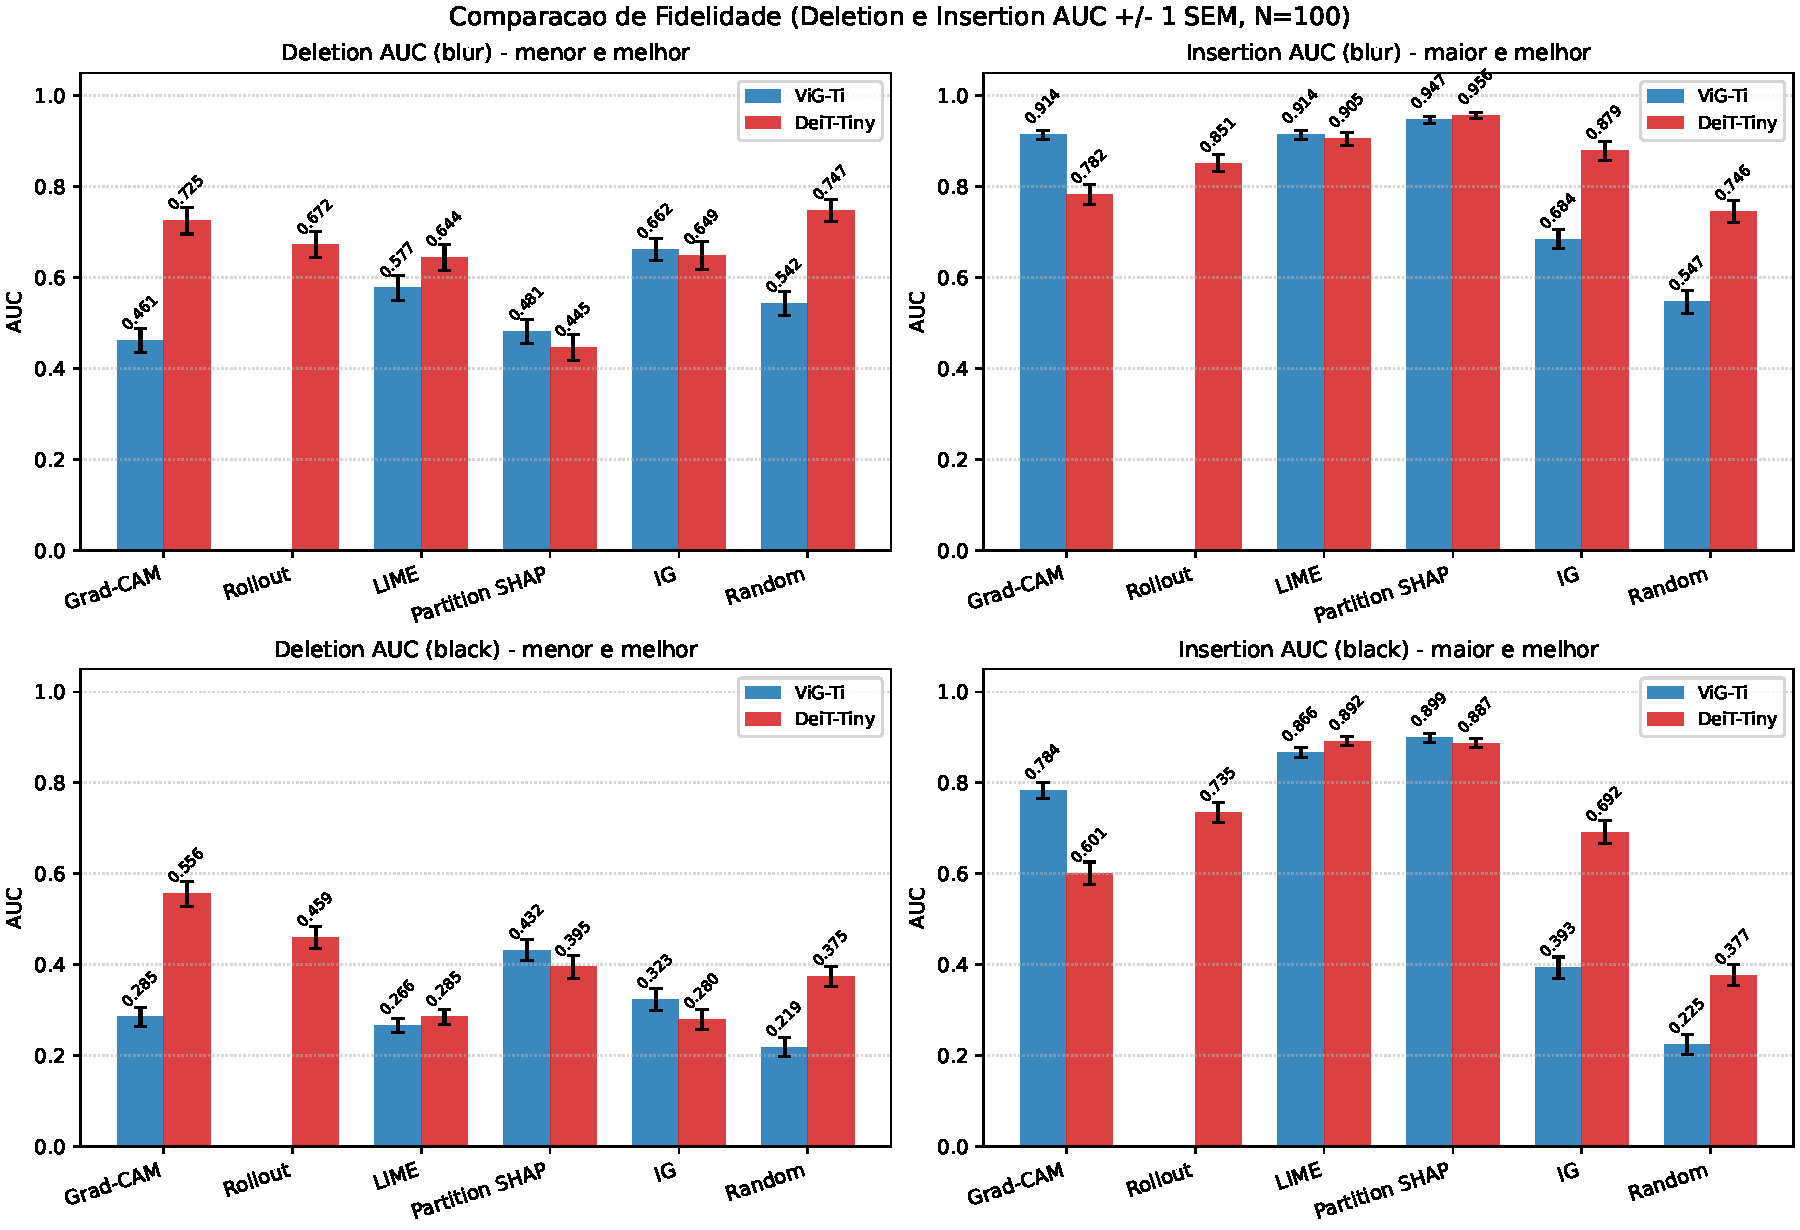
\includegraphics[width=0.84\linewidth]{e3_auc_comparison.pdf}
  \caption{Comparação de Deletion e Insertion AUC ($\pm 1\text{ SEM}$, $N = 100$) sob oclusão \texttt{blur} e \texttt{black} (E3).}
  \label{fig:e3_auc}
\end{figure}

\textbf{Sanity checks, graph rewiring e ruído (E4, E5 e E6):} a Tabela~\ref{tab:e4_e5_e6} e as Figuras~\ref{fig:e4}, \ref{fig:e5} e \ref{fig:e6} sintetizam E4 a E6. Em E4, Grad-CAM, LIME e Partition SHAP colapsam já em \texttt{head}; em contraste, o Rollout mantém Spearman $1{,}000$ em \texttt{head} ($p = 3{,}90 \times 10^{-18}$ vs.\ DeiT Grad-CAM), $0{,}986$ em \texttt{blocks\_9\_11} e $0{,}852$ em \texttt{blocks\_6\_11}, caindo em \texttt{blocks\_3\_11} ($0{,}187$) e \texttt{blocks\_0\_11} ($-0{,}020$). O IG retém Spearman acima de $0{,}41$ em \texttt{all\_layers}, enquanto seu SSIM cai abaixo de $0{,}20$.

Em E5, o Bloco 11 atinge $79\%$ a $83\%$ de \textit{rewiring} com apenas $5\%$ de Deletion e estabiliza em $\approx 85\%$. Sob \texttt{blur}, Partition SHAP ($p = 3{,}03 \times 10^{-7}$) e Grad-CAM ($p = 3{,}06 \times 10^{-4}$) superam \texttt{random} em Rewiring AUC; sob \texttt{black}, \texttt{random} supera todos ($p \le 4{,}36 \times 10^{-6}$). Em $20\%$ de Deletion, o perfil por camada apresenta saltos entre os blocos $3$ e $4$ e entre $7$ e $8$: sob \texttt{blur}, o Grad-CAM sobe de $0{,}208$ (Bloco 0) e $0{,}328$ (Bloco 3) para $0{,}607$ (Bloco 4), $0{,}739$ (Bloco 8) e $0{,}819$ (Bloco 11); sob \texttt{black}, \texttt{random} atinge $0{,}438$ a $0{,}602$ nos blocos $0$ a $3$, contra $0{,}326$ a $0{,}456$ no Grad-CAM e no SHAP.

Em E6, as taxas de inversão de predição ($N = 100$) em $\sigma \in \{0{,}02,\,0{,}05,\,0{,}10\}$ são de $1{,}0\%$, $6{,}0\%$ e $18{,}0\%$ na ViG-Ti contra $1{,}0\%$, $3{,}0\%$ e $4{,}0\%$ no DeiT-Tiny. O DeiT-Tiny supera a ViG-Ti em $\sigma = 0{,}02$ no Grad-CAM ($p = 9{,}07 \times 10^{-16}$), SHAP ($p = 3{,}81 \times 10^{-6}$) e IG ($p = 3{,}90 \times 10^{-18}$), enquanto o LIME colapsa igualmente até $9/20$ mapas constantes em $\sigma = 0{,}10$.

\begin{table}[t]
  \caption{Resultados de \textit{sanity checks} (E4), \textit{graph rewiring} no Bloco 11 (E5) e ruído gaussiano (E6). Em E4 e E6, $N = 100$ para Grad-CAM/Rollout/IG e $N = 20$ para LIME/SHAP.}
  \label{tab:e4_e5_e6}
  \centering
  \resizebox{\linewidth}{!}{%
  \begin{tabular}{llcccccc}
    \toprule
    Modelo & Método & E4 \texttt{head} $\rho$/SSIM & E4 \texttt{all} $\rho$/SSIM & E5 Rew. \texttt{blur}/\texttt{black} & E6 $\rho$ ($0{,}02$) & E6 $\rho$ ($0{,}05$) & E6 $\rho$ ($0{,}10$) \\
    \midrule
    ViG-Ti & Grad-CAM & $-0{,}015 / 0{,}407$ & $0{,}027 / 0{,}326$ & $0{,}812 / 0{,}824$ & $0{,}782$ & $0{,}697$ & $0{,}557$ \\
    ViG-Ti & LIME & $-0{,}068 / 0{,}412$ & $-0{,}053 / 0{,}393$ & $0{,}811 / 0{,}823$ & $0{,}565$ & $0{,}224$ & $0{,}036$ \\
    ViG-Ti & Partition SHAP & $-0{,}249 / 0{,}350$ & $-0{,}140 / 0{,}386$ & $0{,}813 / 0{,}823$ & $0{,}734$ & $0{,}601$ & $0{,}340$ \\
    ViG-Ti & IG & $0{,}583 / 0{,}466$ & $0{,}430 / 0{,}192$ & $0{,}806 / 0{,}830$ & $0{,}552$ & $0{,}535$ & $0{,}509$ \\
    ViG-Ti & Random &  &  & $0{,}810 / 0{,}831$ &  &  &  \\
    \midrule
    DeiT-Tiny & Grad-CAM & $-0{,}067 / 0{,}175$ & $-0{,}019 / 0{,}176$ &  & $0{,}935$ & $0{,}805$ & $0{,}611$ \\
    DeiT-Tiny & Rollout & $1{,}000 / 1{,}000$ & $-0{,}024 / 0{,}353$ &  & $0{,}994$ & $0{,}959$ & $0{,}882$ \\
    DeiT-Tiny & LIME & $-0{,}023 / 0{,}451$ & $-0{,}136 / 0{,}405$ &  & $0{,}504$ & $0{,}223$ & $0{,}056$ \\
    DeiT-Tiny & Partition SHAP & $-0{,}011 / 0{,}520$ & $0{,}059 / 0{,}549$ &  & $0{,}938$ & $0{,}822$ & $0{,}676$ \\
    DeiT-Tiny & IG & $0{,}698 / 0{,}656$ & $0{,}419 / 0{,}164$ &  & $0{,}923$ & $0{,}838$ & $0{,}748$ \\
    \bottomrule
  \end{tabular}}
\end{table}

\begin{figure}[t]
  \centering
  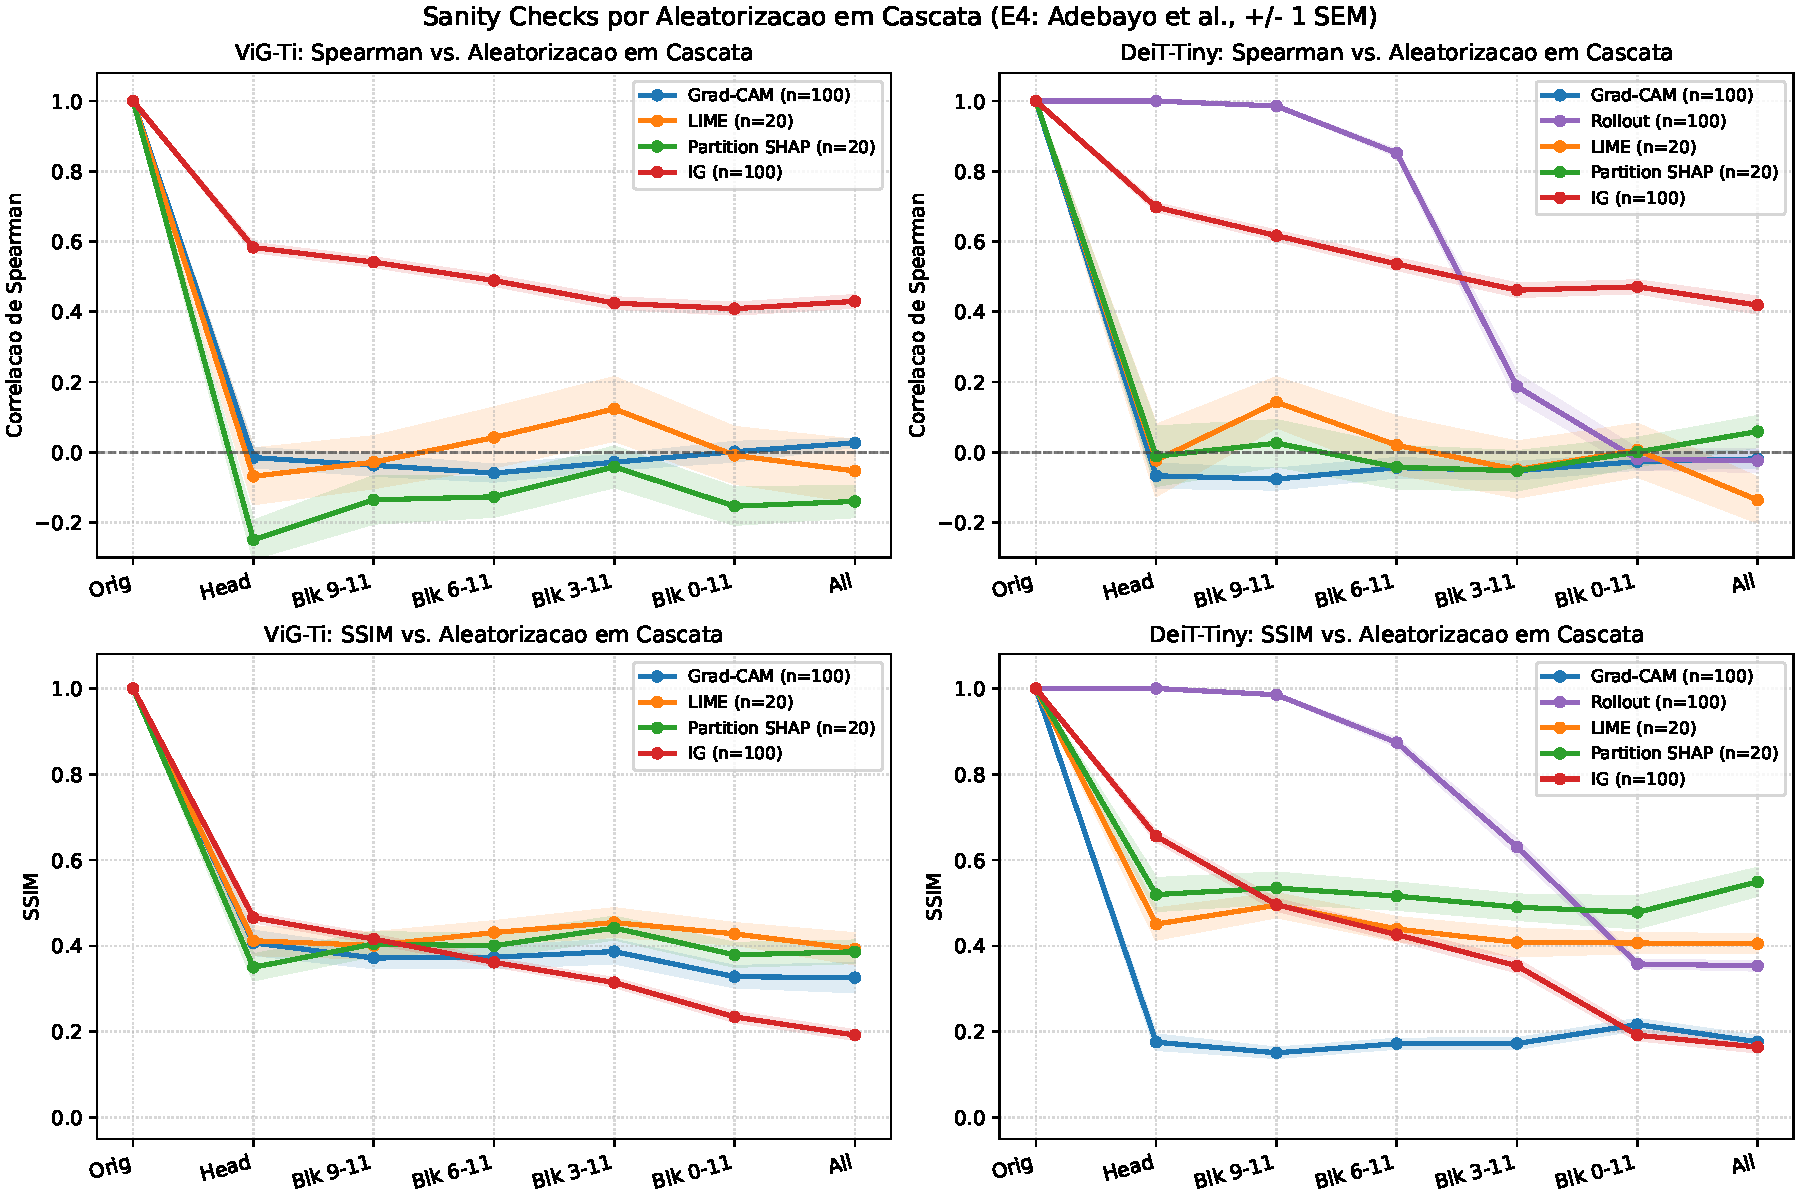
\includegraphics[width=0.84\linewidth]{e4_sanity_curves.pdf}
  \caption{Aleatorização em cascata de \texttt{Head} até \texttt{All} medida por Spearman e SSIM ($\pm 1\text{ SEM}$, E4).}
  \label{fig:e4}
\end{figure}

\begin{figure}[t]
  \centering
  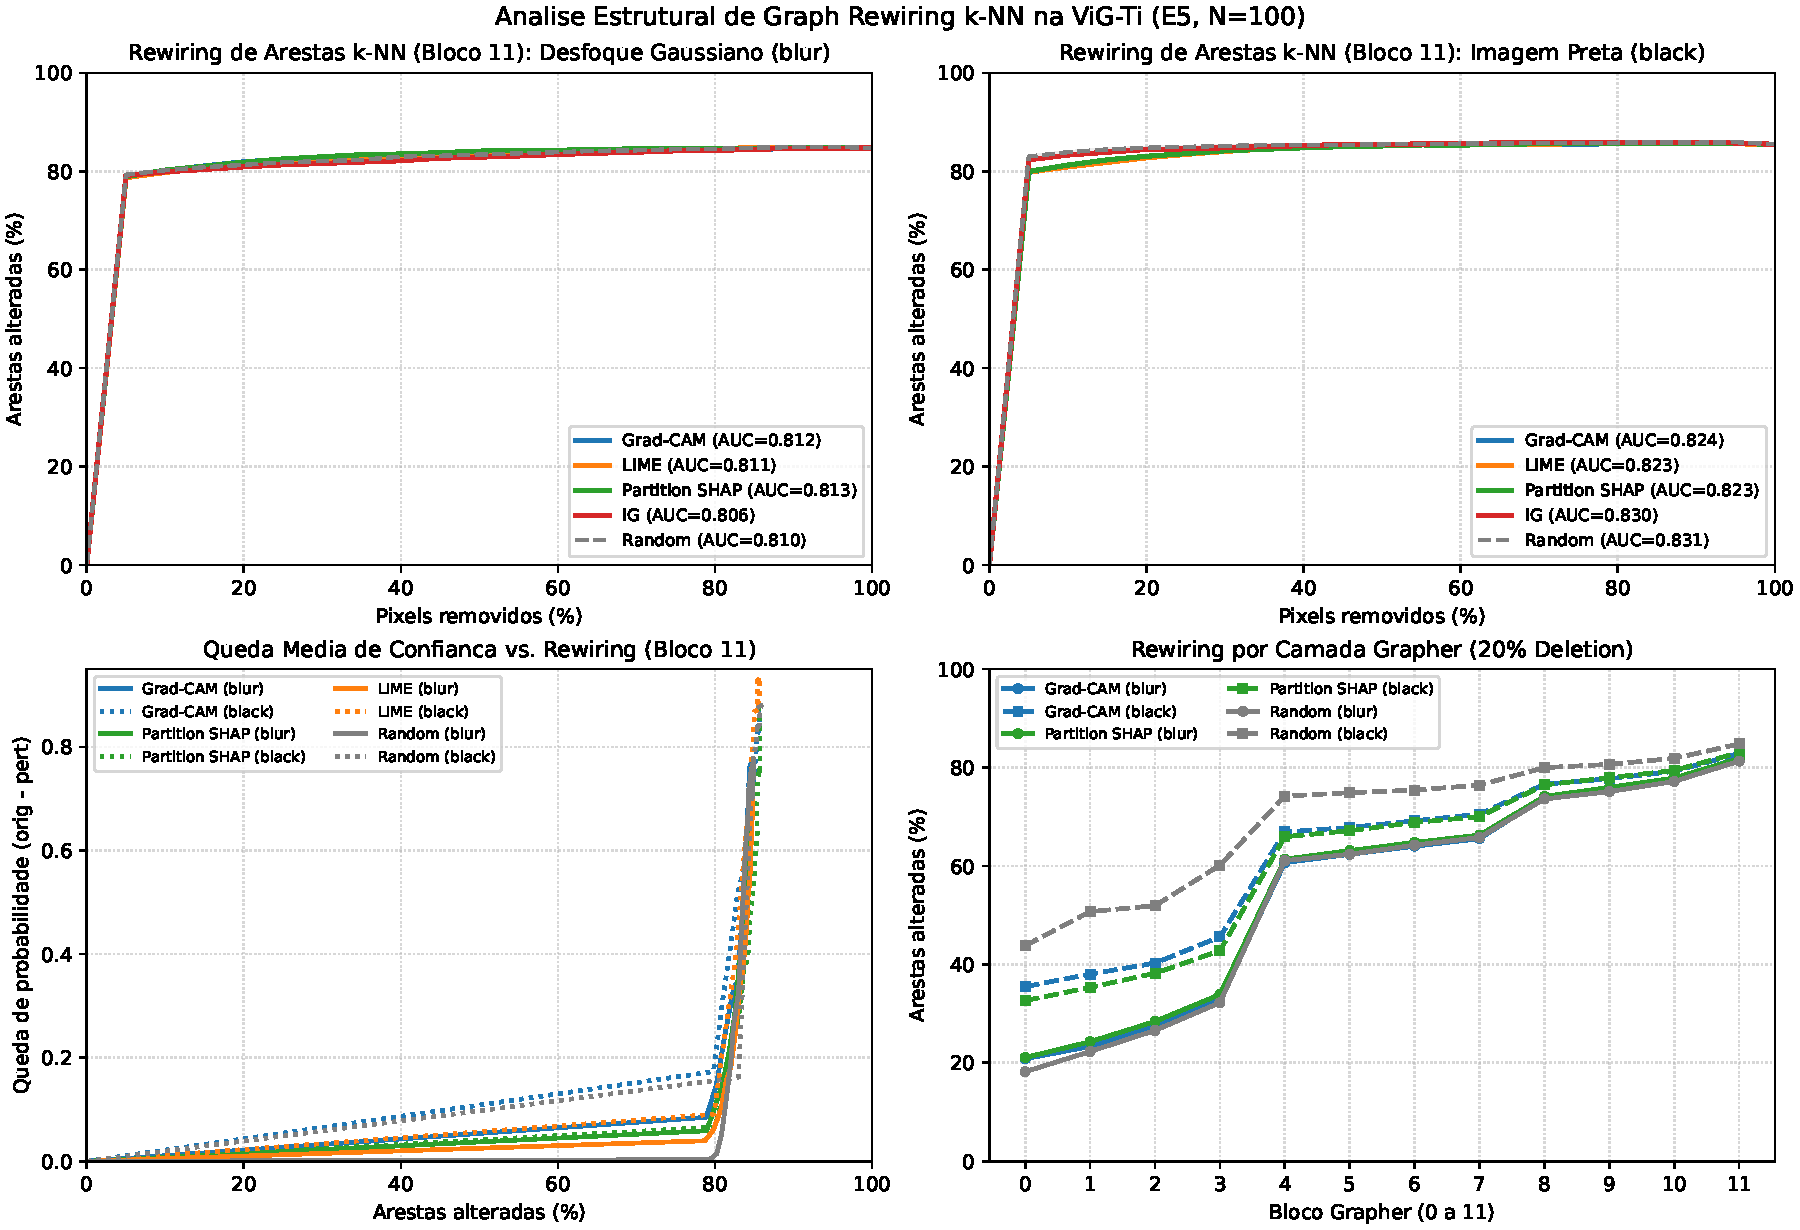
\includegraphics[width=0.84\linewidth]{e5_graph_rewiring.pdf}
  \caption{\textit{Graph rewiring} $k$-NN na ViG-Ti (E5, $N = 100$): Bloco 11 sob \texttt{blur}/\texttt{black}, queda de confiança e perfil nos $12$ blocos em $20\%$ de Deletion.}
  \label{fig:e5}
\end{figure}

\begin{figure}[t]
  \centering
  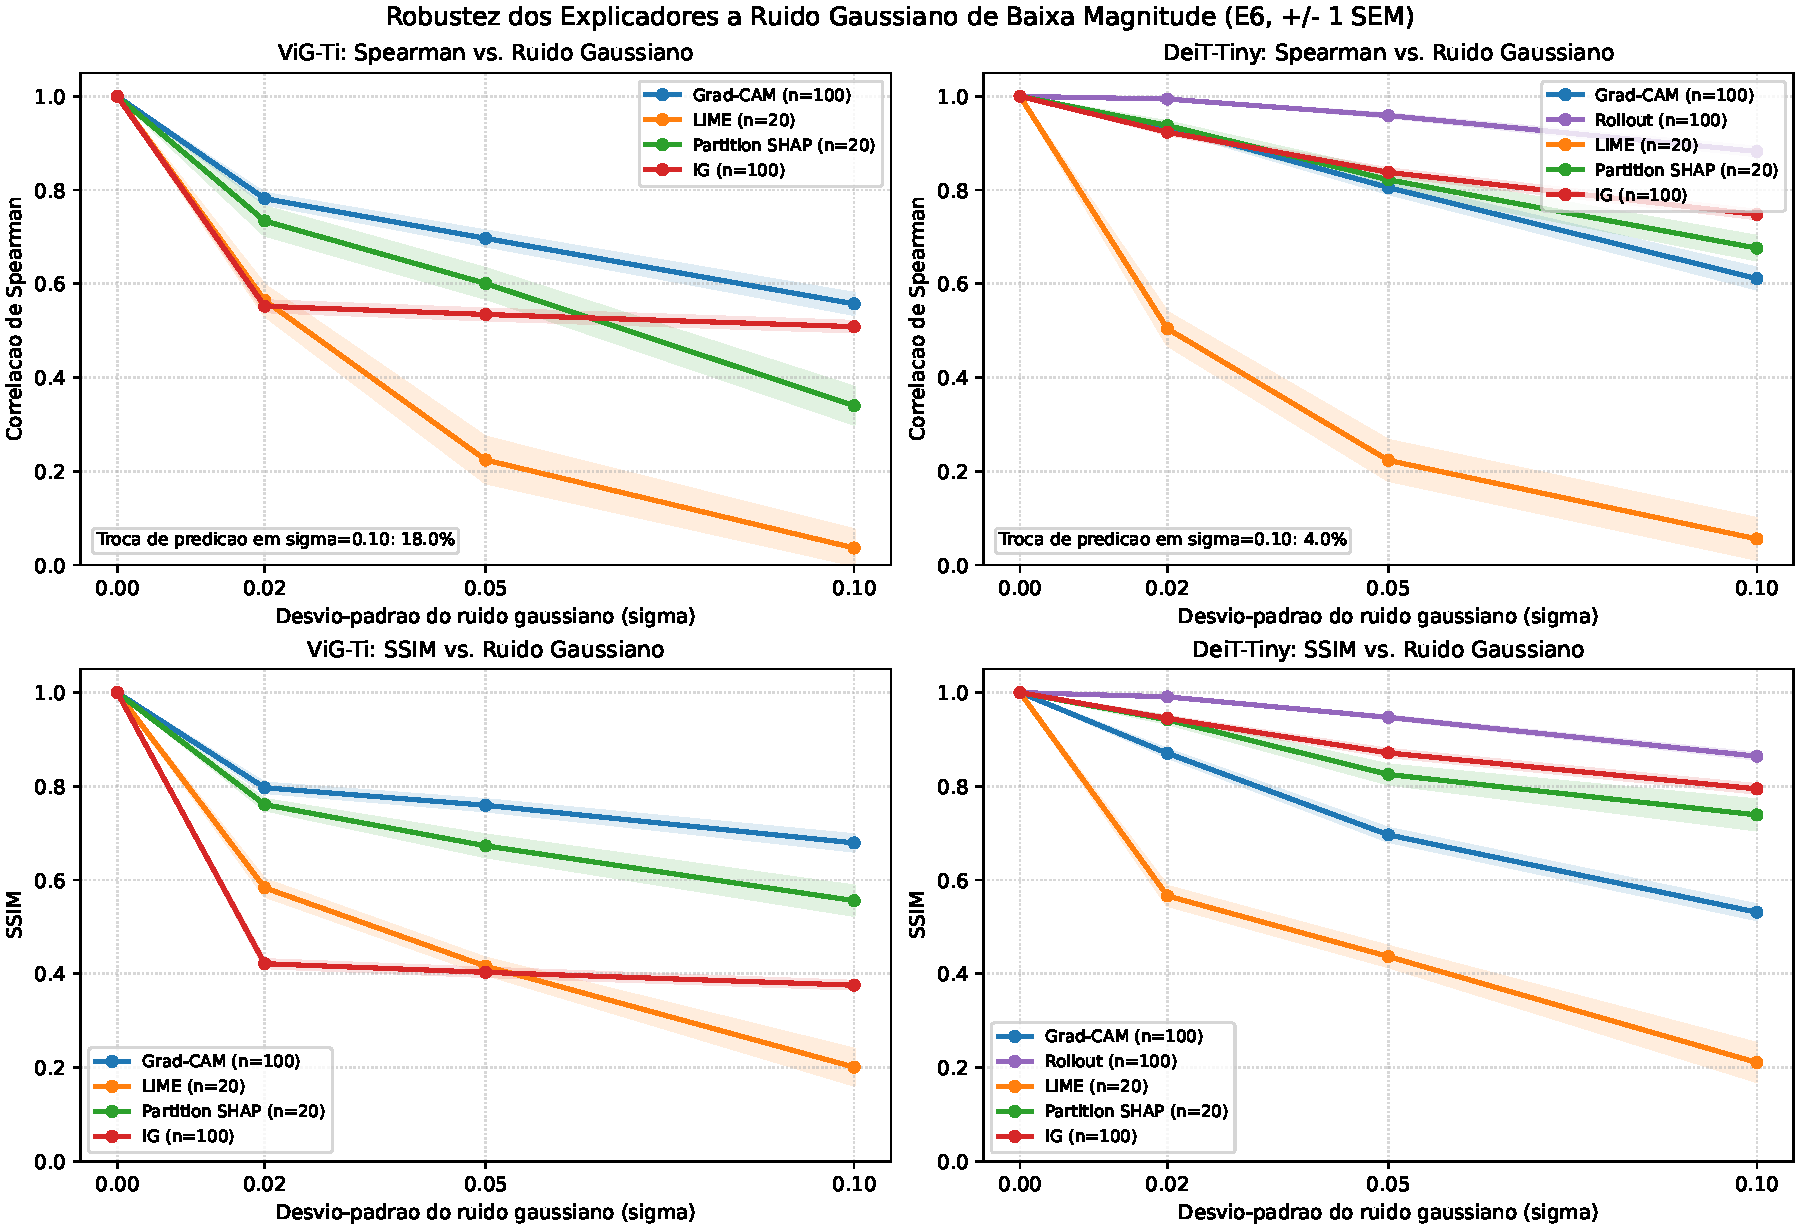
\includegraphics[width=0.84\linewidth]{e6_noise_robustness.pdf}
  \caption{Estabilidade sob ruído gaussiano ($\sigma \in \{0{,}02,\,0{,}05,\,0{,}10\}$) e troca de predição em $\sigma = 0{,}10$ (E6).}
  \label{fig:e6}
\end{figure}

\textbf{Ablações e inspeção qualitativa:} na Figura~\ref{fig:ablation} ($N = 20$, \texttt{blur}), variar \texttt{n\_segments} no LIME ($25, 50, 100$) muda a segmentação (Spearman $0{,}308$ a $0{,}412$ contra $50$), mantendo Insertion AUC em $0{,}880$ a $0{,}939$ (ViG-Ti) e $0{,}897$ a $0{,}904$ (DeiT-Tiny). No IG (\texttt{n\_steps} $\in \{20, 50, 100\}$), o DeiT-Tiny mantém Spearman $0{,}949$ ($20$) e $0{,}994$ ($100$) contra $50$ passos, enquanto a ViG-Ti varia mais ($0{,}559$ e $0{,}719$), com AUCs médios estáveis ($0{,}639$ a $0{,}692$). Nos $3$ erros por modelo em \texttt{xai\_subset.csv}, a confiança inicial é menor ($0{,}575$ e $0{,}752$) que nos $97$ acertos ($0{,}988$ e $0{,}993$), e o Deletion AUC (\texttt{blur}) do Grad-CAM cai para $0{,}085$ e $0{,}076$. As Figuras~\ref{fig:errors} e \ref{fig:divergence} ilustram os $4$ casos de erro/discordância e $3$ divergências entre plausibilidade e métricas E3/E4.

\begin{figure}[t]
  \centering
  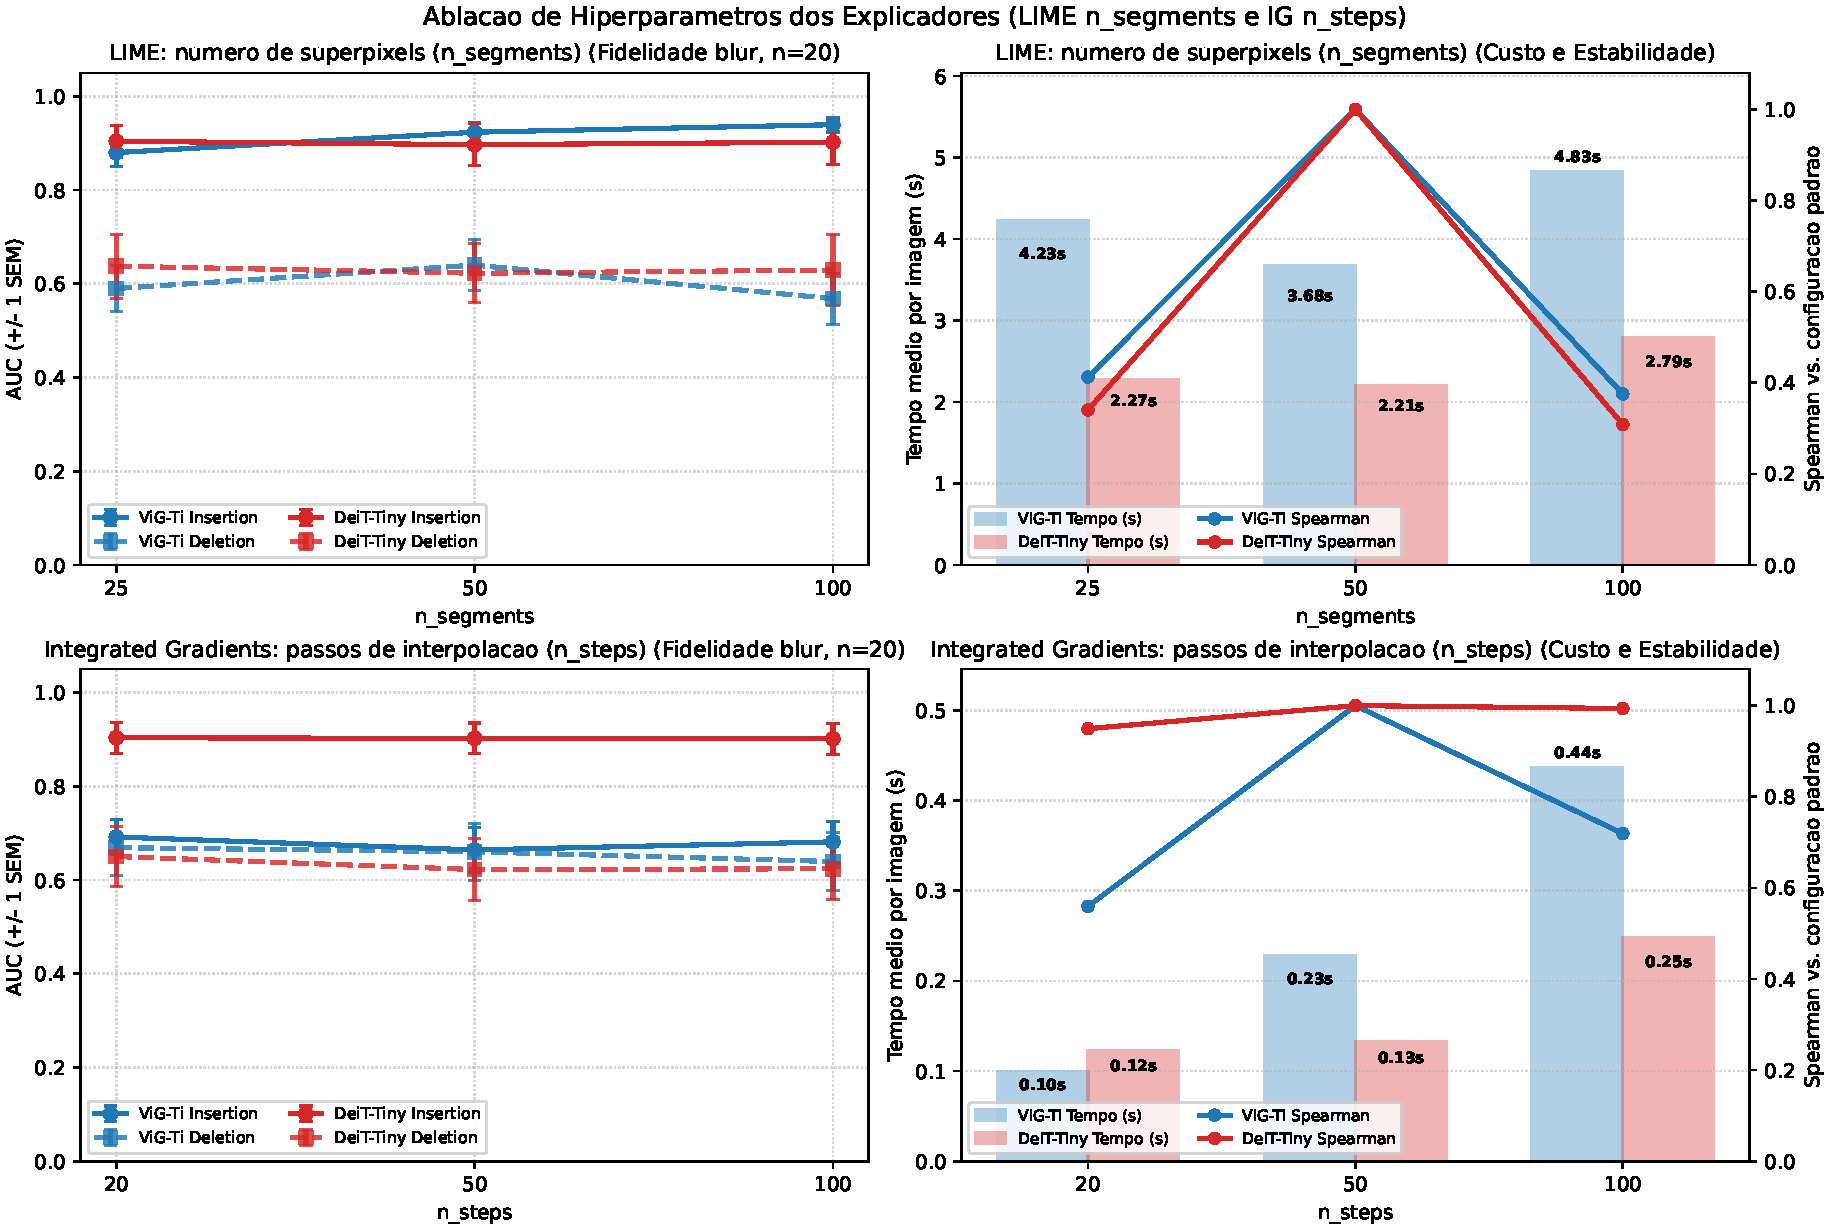
\includegraphics[width=0.84\linewidth]{ablation_sensitivity.pdf}
  \caption{Sensibilidade de fidelidade (\texttt{blur}), tempo médio e Spearman para LIME e IG ($N = 20$).}
  \label{fig:ablation}
\end{figure}

\begin{figure}[t]
  \centering
  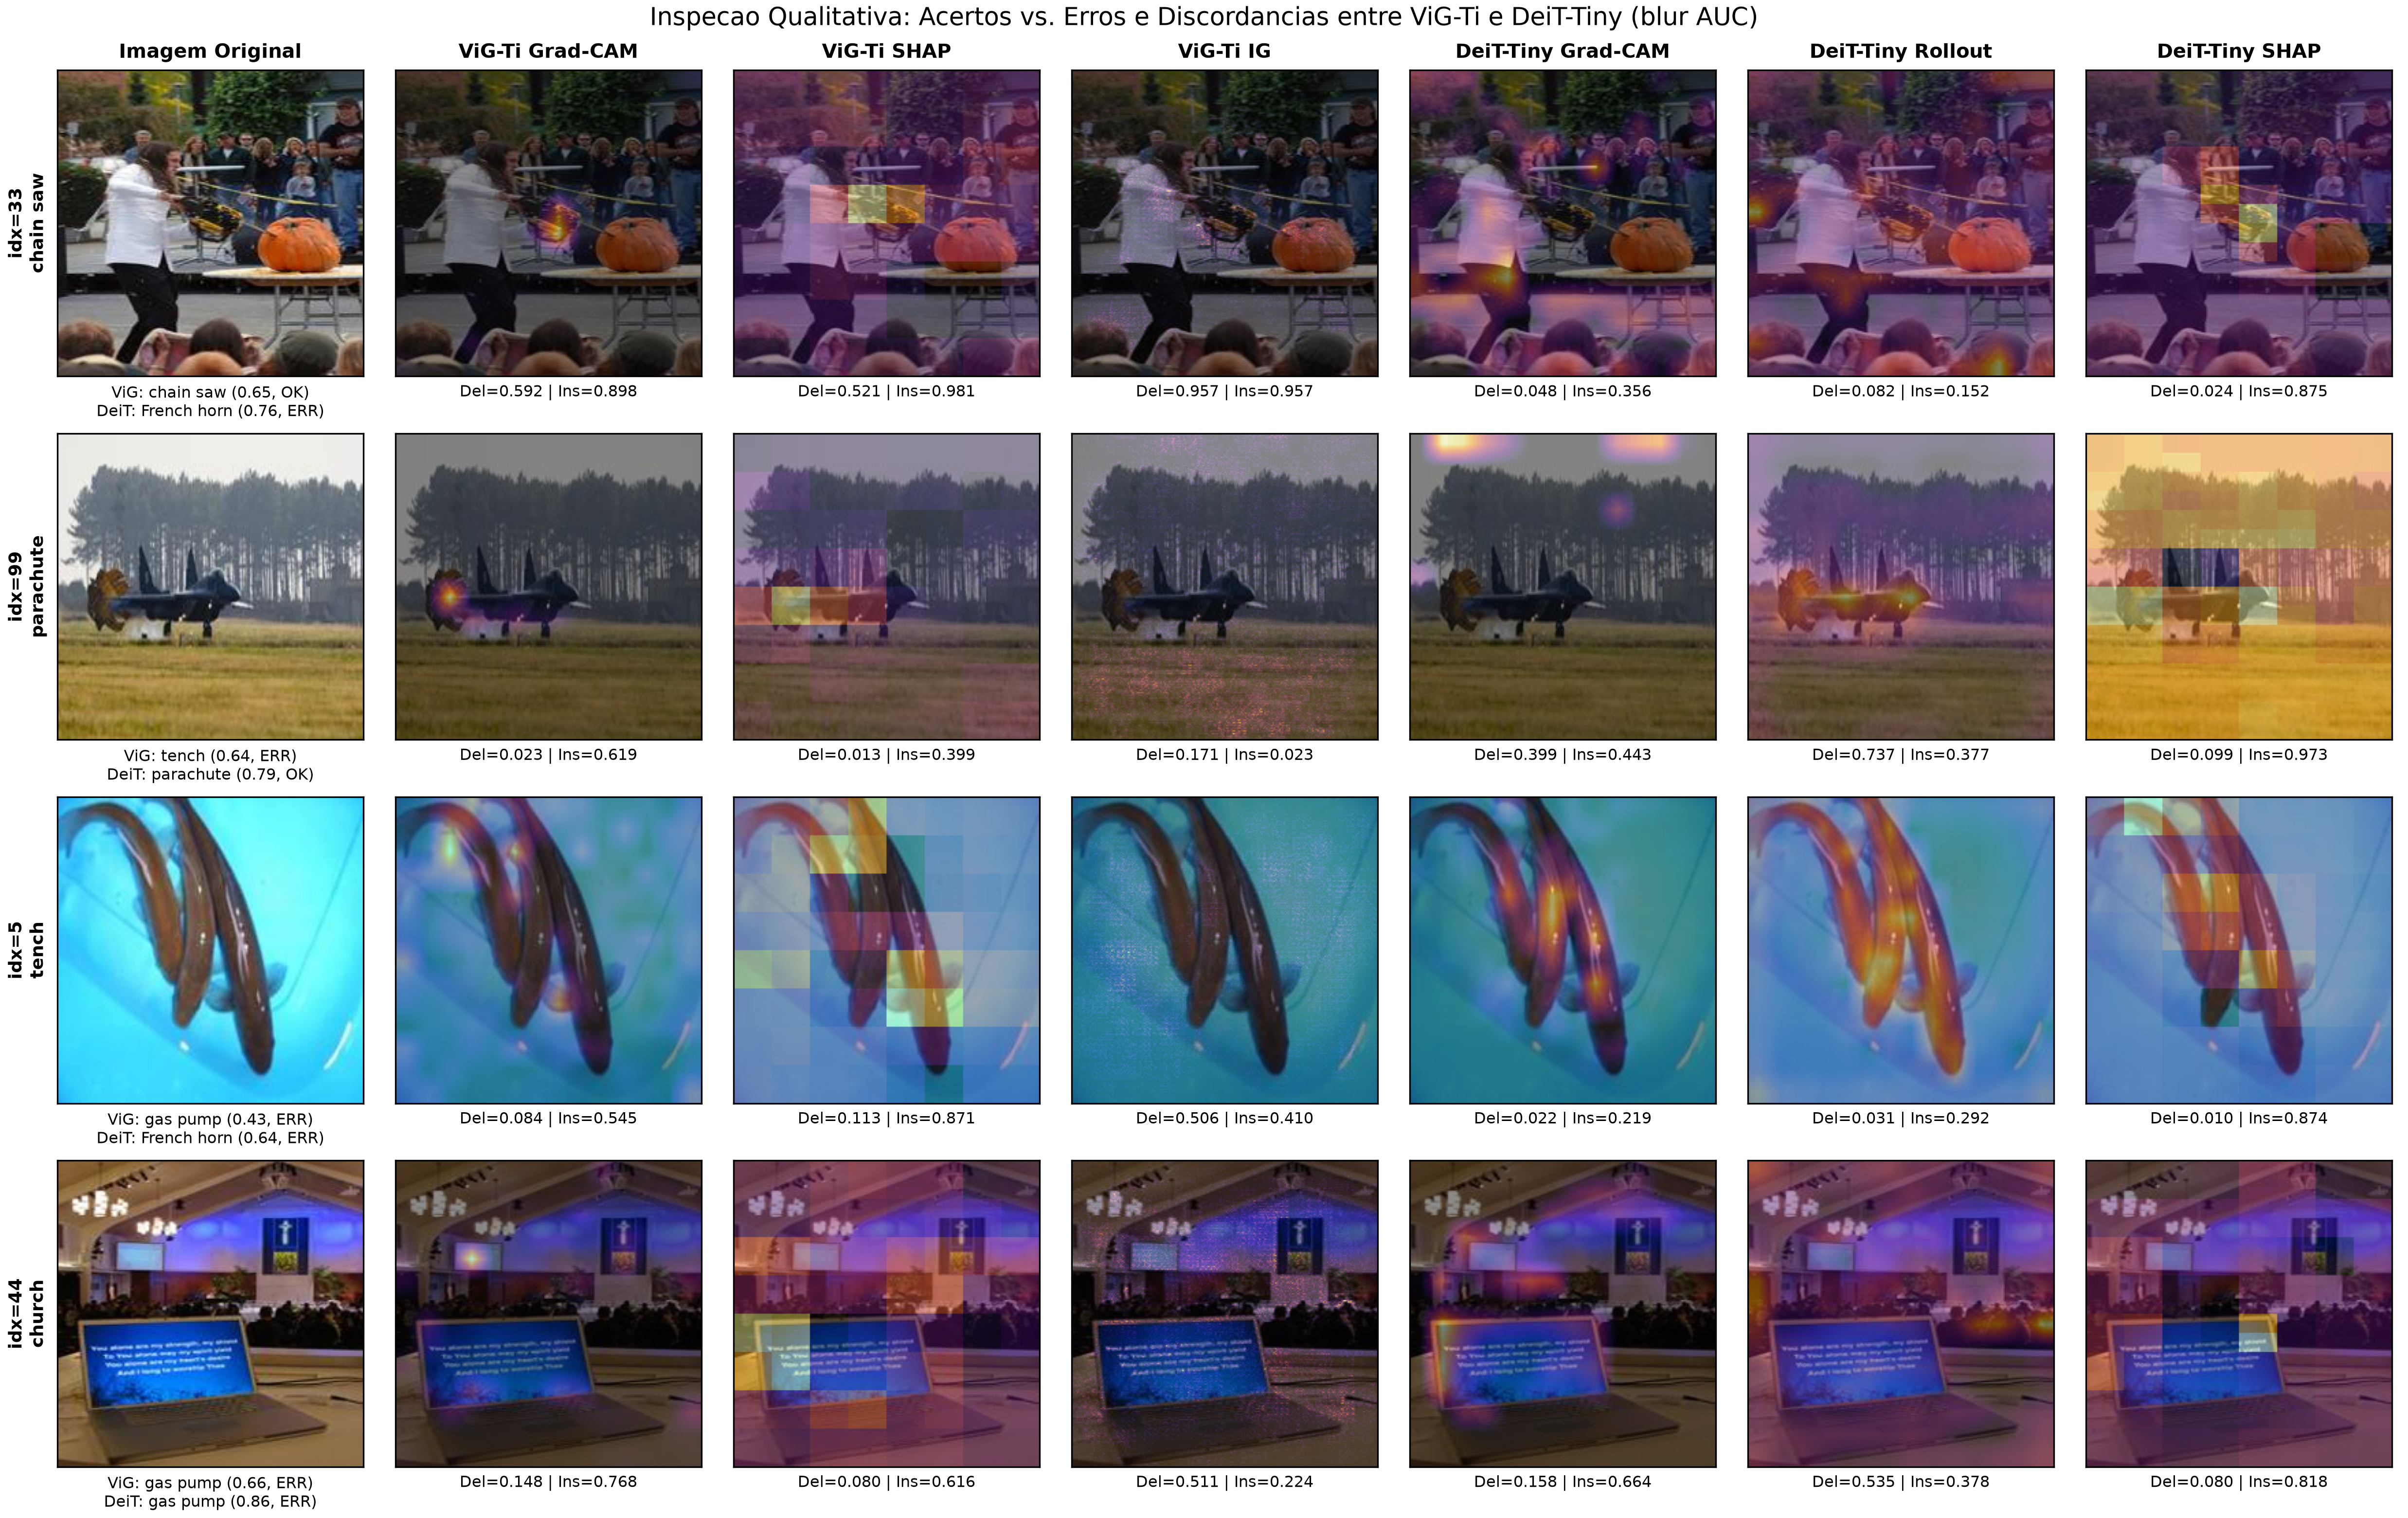
\includegraphics[width=0.96\linewidth]{analysis_errors_vs_correct.png}
  \caption{Estudos de caso nos $4$ exemplos com erro ou discordância no \texttt{xai\_subset.csv} (\texttt{blur} AUC).}
  \label{fig:errors}
\end{figure}

\begin{figure}[t]
  \centering
  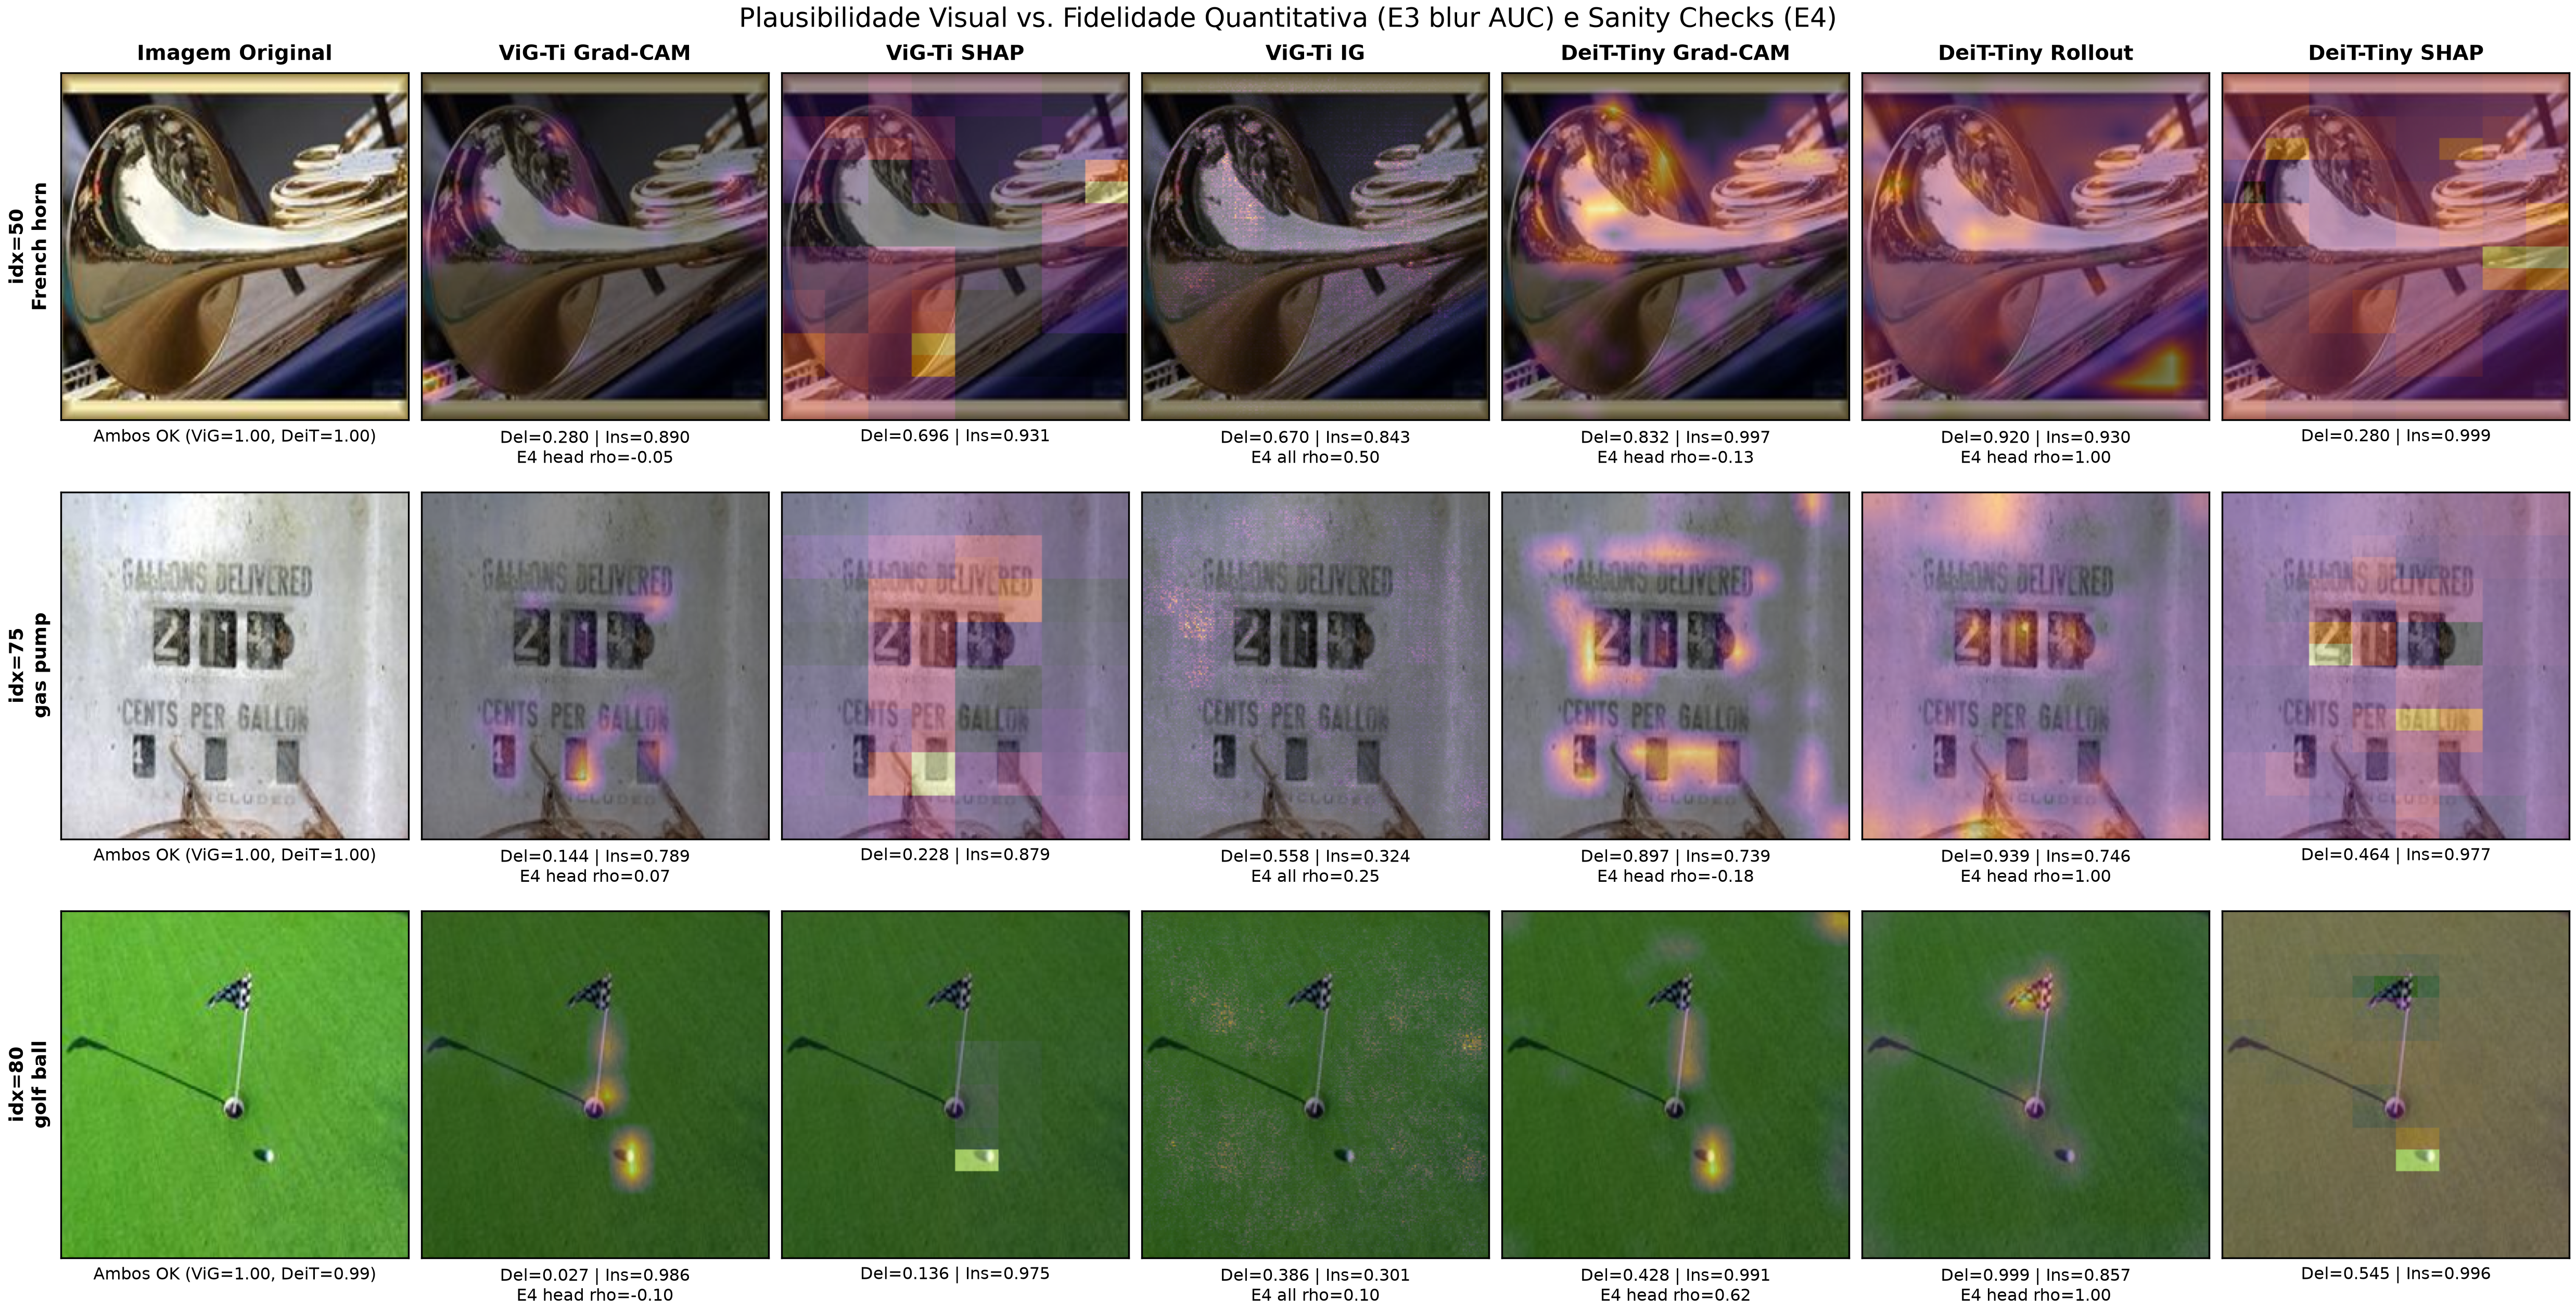
\includegraphics[width=0.96\linewidth]{analysis_plausibility_vs_faithfulness.png}
  \caption{Divergência entre plausibilidade visual e métricas (E3 \texttt{blur} AUC e E4 Spearman).}
  \label{fig:divergence}
\end{figure}

\section{Discussion}
\label{sec:discussion}
% O que escrever aqui:
% - Interpretem os resultados da Seção \ref{sec:results}: o que eles
%   significam em relação à pergunta de pesquisa?
% - Comparem com o baseline e com a literatura discutida em Related Work.
% - Casos de erro/falha interessantes, se houver.

\textbf{Superioridade do Grad-CAM na ViG-Ti vs.\ DeiT-Tiny:} na ViG-Ti, os $196$ nós de \texttt{backbone[-1]} seguem diretamente para o \textit{global average pooling}, preservando ligação causal direta entre gradiente e predição. No DeiT-Tiny, apenas o \textit{token} \texttt{CLS} alimenta o cabeçalho de classificação, permitindo que \textit{tokens} espaciais de borda e fundo em \texttt{blocks[-1].norm1} acumulem norma elevada \citep{darcet2024registers}, degradando o Grad-CAM em E3 em comparação tanto à ViG-Ti quanto ao Attention Rollout.

\textbf{Plausibilidade visual e estabilidade vs.\ fidelidade:} o Rollout do DeiT-Tiny é visualmente limpo e o mais estável em E6 ($0{,}882$ em $\sigma = 0{,}10$), porém é completamente insensível ao cabeçalho em E4 (\texttt{head} $= 1{,}000$), confirmando \citet{chefer2021transformer} e \citet{adebayo2018sanity}. Em \texttt{idx=80} (\textit{golf ball}, Figura~\ref{fig:divergence}), o Rollout marca a bandeira com nitidez, mas deixa o modelo confiante até quase $100\%$ de oclusão (\texttt{Del} $= 0{,}999$), enquanto o Grad-CAM da ViG-Ti isola a bola e o buraco (\texttt{Del} $= 0{,}027$). Em \texttt{idx=50} e \texttt{idx=75}, o Grad-CAM do DeiT-Tiny parece coerente, mas atinge \texttt{Del} $= 0{,}832$ e $0{,}897$. No IG, o fator $(x - x')$ explica a retenção de Spearman ($\approx 0{,}42$ a $0{,}43$) em \texttt{all\_layers} \citep{adebayo2018sanity}, enquanto a inversão em Insertion AUC ($0{,}879$ no DeiT-Tiny vs.\ $0{,}684$ na ViG-Ti) reflete que pontos isolados já ativam a projeção linear de \textit{patches} do ViT, mas não o \textit{Stem} convolucional com \texttt{BatchNorm2d}.

\textbf{Mecanismo do grafo $k$-NN (E3, E5, E6 e ablações):} em E5, pixels pretos aleatórios (\texttt{black}) corrompem quase todos os \textit{patches} iniciais, gerando $43{,}8\%$ a $60{,}2\%$ de \textit{rewiring} nos blocos $0$ a $3$ em $20\%$ de Deletion (contra $32{,}6\%$ a $45{,}6\%$ em Grad-CAM e SHAP) e explicando o falso bom Deletion de \texttt{random} ($0{,}219$) em E3. Sob \texttt{blur}, explicadores reais superam \texttt{random} tanto em Deletion quanto em \textit{rewiring}. Os saltos entre os blocos $4$ e $8$ acompanham o aumento da dilatação ($d = 1 \rightarrow 2 \rightarrow 3$), e o platô de $\approx 85{,}5\%$ no Bloco 11 reflete o teto teórico ($\approx 86{,}2\%$) imposto pelo \textit{self-loop} $(i, i)$ na posição $0$ do \texttt{DenseDilatedKnnGraph} ($1/18 = 5{,}56\%$ das arestas). Em contrapartida, a operação discreta de \texttt{topk} torna a ViG-Ti sensível a TF32 entre lotes em E1/E2, produz maior taxa de inversão de predição e queda de correlação sob ruído em E6 ($18{,}0\%$ vs.\ $4{,}0\%$ em $\sigma = 0{,}10$; IG Spearman $0{,}552$ em $\sigma = 0{,}02$) e maior variação do IG com \texttt{n\_steps} ($0{,}559$ e $0{,}719$ na ViG-Ti vs.\ $0{,}949$ e $0{,}994$ no DeiT-Tiny). No LIME em E6, o colapso idêntico em ambos os modelos ($9/20$ mapas constantes exatamente nas mesmas imagens em $\sigma = 0{,}10$) decorre da degradação do SLIC no espaço CIELAB, cuja mediana de superpixels cai de $34{,}5$ ($\sigma = 0{,}00$) para $10{,}5$ ($\sigma = 0{,}05$) e $2{,}0$ ($\sigma = 0{,}10$).

\textbf{Casos qualitativos de acertos e erros (Figura~\ref{fig:errors}):} em \texttt{idx=33} (\textit{chain saw}), acerto exclusivo da ViG-Ti, seu Grad-CAM foca na motosserra, enquanto o do DeiT-Tiny (que previu \textit{French horn}) ativa os espectadores na borda inferior. Em \texttt{idx=44} (\textit{church}), ambos erram prevendo \textit{gas pump} ao focar na tela iluminada do laptop em primeiro plano. Em \texttt{idx=99} (\textit{parachute}), acerto exclusivo do DeiT-Tiny, o Rollout cobre parte do paraquedas de frenagem, enquanto a ViG-Ti ativa a extremidade traseira com confiança moderada ($0{,}64$) na classe errada (\textit{tench}). Entre os métodos agnósticos, o Partition SHAP oferece o melhor equilíbrio nas duas arquiteturas.

\section{Limitations}
\label{sec:limitations}
% O que escrever aqui:
% - Limitações dos dados, do método ou da avaliação.
% - O que não foi possível testar por restrições de tempo/recursos.
% - Ameaças à validade dos resultados (ex.: tamanho da amostra,
%   generalização, vazamento de dados).

Avaliou-se apenas o \texttt{imagenette2-160} ($10$ classes) e um par isotrópico compacto, resultando em apenas $3$ erros por modelo em $N = 100$ e restringindo a análise de erros a estudos de caso. Pelo custo do LIME e do Partition SHAP, E4, E6 e ablações usaram $N = 20$ imagens estratificadas para métodos por perturbação. Além disso, métricas sem retreino \citep{petsiuk2018rise}, ao contrário do ROAR \citep{hooker2019roar}, sofrem influência da base residual de \texttt{blur} ($0{,}517$ no DeiT-Tiny vs.\ $0{,}271$ na ViG-Ti). Não foram incluídos ViTs com \textit{register tokens} \citep{darcet2024registers}, variantes piramidais nem atribuição ponderada por gradientes em Transformers \citep{chefer2021transformer}.

\section{Conclusion}
\label{sec:conclusion}
% O que escrever aqui:
% - Retomem a pergunta de pesquisa e respondam-na com base nos resultados.
% - Principais conclusões do trabalho, em 3 a 5 frases.
% - Trabalhos futuros: o que fariam com mais tempo/recursos.

Respondendo à pergunta de pesquisa, métodos de XAI \textit{post-hoc} não preservam o mesmo grau de fidelidade e estabilidade entre a ViG-Ti e o DeiT-Tiny, mesmo sob paridade de acurácia, profundidade e largura. A conectividade esparsa local da ViG-Ti favorece o Grad-CAM em fidelidade, mas o \textit{topk} discreto aumenta a sensibilidade a oclusão por preto, ruído gaussiano e discretização do caminho de integração. No DeiT-Tiny, o \textit{self-attention} denso garante maior estabilidade a ruído e melhor Insertion no IG, porém contamina o Grad-CAM com \textit{tokens} de borda, enquanto o Attention Rollout falha no \textit{sanity check} do cabeçalho. O Partition SHAP apresentou a maior consistência cruzada. Trabalhos futuros devem incluir ViTs com \textit{register tokens}, propagação de relevância com gradiente e grafos $k$-NN diferenciáveis.

\clearpage
\bibliographystyle{plainnat}
\bibliography{references}

\end{document}
